
% LaTeX Beamer file automatically generated from DocOnce
% https://github.com/hplgit/doconce

%-------------------- begin beamer-specific preamble ----------------------

\documentclass{beamer}

\usetheme{red_shadow}
\usecolortheme{default}

% turn off the almost invisible, yet disturbing, navigation symbols:
\setbeamertemplate{navigation symbols}{}

% Exemples on customization:
%\usecolortheme[named=RawSienna]{structure}
%\usetheme[height=7mm]{Rochester}
%\setbeamerfont{frametitle}{family=\rmfamily,shape=\itshape}
%\setbeamertemplate{items}[ball]
%\setbeamertemplate{blocks}[rounded][shadow=true]
%\useoutertheme{infolines}
%
%\usefonttheme{}
%\useinntertheme{}
%
%\setbeameroption{show notes}
%\setbeameroption{show notes on second screen=right}

% fine for B/W printing:
%\usecolortheme{seahorse}

\usepackage{pgf}
\usepackage{graphicx}
\usepackage{epsfig}
\usepackage{relsize}

\usepackage{fancybox}  % make sure fancybox is loaded before fancyvrb

\usepackage{fancyvrb}
\usepackage{minted} % requires pygments and latex -shell-escape filename
%\usepackage{anslistings}
%\usepackage{listingsutf8}

\usepackage{amsmath,amssymb,bm}
%\usepackage[latin1]{inputenc}
\usepackage[T1]{fontenc}
\usepackage[utf8]{inputenc}
\usepackage{colortbl}
\usepackage[english]{babel}
\usepackage{tikz}
\usepackage{framed}
% Use some nice templates
\beamertemplatetransparentcovereddynamic

% --- begin table of contents based on sections ---
% Delete this, if you do not want the table of contents to pop up at
% the beginning of each section:
% (Only section headings can enter the table of contents in Beamer
% slides generated from DocOnce source, while subsections are used
% for the title in ordinary slides.)
\AtBeginSection[]
{
  \begin{frame}<beamer>[plain]
  \frametitle{}
  %\frametitle{Outline}
  \tableofcontents[currentsection]
  \end{frame}
}
% --- end table of contents based on sections ---

% If you wish to uncover everything in a step-wise fashion, uncomment
% the following command:

%\beamerdefaultoverlayspecification{<+->}

\newcommand{\shortinlinecomment}[3]{\note{\textbf{#1}: #2}}
\newcommand{\longinlinecomment}[3]{\shortinlinecomment{#1}{#2}{#3}}

\definecolor{linkcolor}{rgb}{0,0,0.4}
\hypersetup{
    colorlinks=true,
    linkcolor=linkcolor,
    urlcolor=linkcolor,
    pdfmenubar=true,
    pdftoolbar=true,
    bookmarksdepth=3
    }
\setlength{\parskip}{7pt}  % {1em}

\newenvironment{doconceexercise}{}{}
\newcounter{doconceexercisecounter}
\newenvironment{doconce:movie}{}{}
\newcounter{doconce:movie:counter}

\newcommand{\subex}[1]{\noindent\textbf{#1}}  % for subexercises: a), b), etc

\logo{{\tiny \copyright\ 2019, Ahmed Ammar. Released under CC Attribution 4.0 license}}

%-------------------- end beamer-specific preamble ----------------------

% Add user's preamble




% insert custom LaTeX commands...

\raggedbottom
\makeindex

%-------------------- end preamble ----------------------

\begin{document}

% matching end for #ifdef PREAMBLE

\newcommand{\exercisesection}[1]{\subsection*{#1}}



% ------------------- main content ----------------------



% ----------------- title -------------------------

\title{Tutoriel: Apprendre l'Astronomie avec Python}

% ----------------- author(s) -------------------------

\author{Ahmed Ammar\inst{1}}
\institute{Faculté des Sciences, Université de Tunis El Manar et Société Astronomique de Tunisie.\inst{1}}
% ----------------- end author(s) -------------------------

\date{2019
% <optional titlepage figure>
\ \\ 
{\tiny \copyright\ 2019, Ahmed Ammar. Released under CC Attribution 4.0 license}
}

\begin{frame}[plain,fragile]
\titlepage
\end{frame}

\section{Python}

\begin{frame}[plain,fragile]
\frametitle{Python}

\href{{http://www.python.org/}}{Python} est un langage de programmation moderne de haut niveau, orienté objet et d'usage général.

\textbf{Caractéristiques générales de Python} :

\begin{itemize}
\item Langage simple:
\begin{itemize}

  \item facile à lire et à apprendre avec une syntaxe minimaliste.

\end{itemize}

\noindent
\item Langage concis et expressif:
\begin{itemize}

  \item moins de lignes de code

  \item moins de bugs

  \item plus facile à maintenir.
\end{itemize}

\noindent
\end{itemize}

\noindent

\end{frame}

\begin{frame}[plain,fragile]
% No title on this slide

\textbf{Détails techniques} :

\begin{itemize}
\item Typé dynamiquement:
\begin{itemize}

  \item Pas besoin de définir le type des variables, les arguments ou le type des fonctions.

\end{itemize}

\noindent
\item La gestion automatique de la mémoire:
\begin{itemize}

  \item Aucune nécessité d'allouer explicitement et désallouer la mémoire pour les variables et les tableaux de données. Aucun bug de fuite de mémoire.

\end{itemize}

\noindent
\item Interprété:
\begin{itemize}

  \item Pas besoin de compiler le code. L'interpréteur Python lit et exécute le code python directement.
\end{itemize}

\noindent
\end{itemize}

\noindent
\end{frame}

\begin{frame}[plain,fragile]
% No title on this slide

\textbf{Avantages} :

\begin{itemize}
\item Le principal avantage est la facilité de programmation, qui minimise le temps nécessaire pour développer, déboguer et maintenir le code.

\item Langage bien conçu qui encourage les bonnes pratiques de programmation:
\begin{itemize}

  \item Modulaire et orientée objet, permet l'encapsulation  et la réutilisation de code. Il en résulte souvent un code plus transparent, plus facile à améliorer et sans bug.

  \item Documentation intégré avec le code.

\end{itemize}

\noindent
\item De nombreuses bibliothèques standards, et de nombreux packages add-on.
\end{itemize}

\noindent
\end{frame}

\begin{frame}[plain,fragile]
% No title on this slide

\vspace{6mm}

% inline figure
\centerline{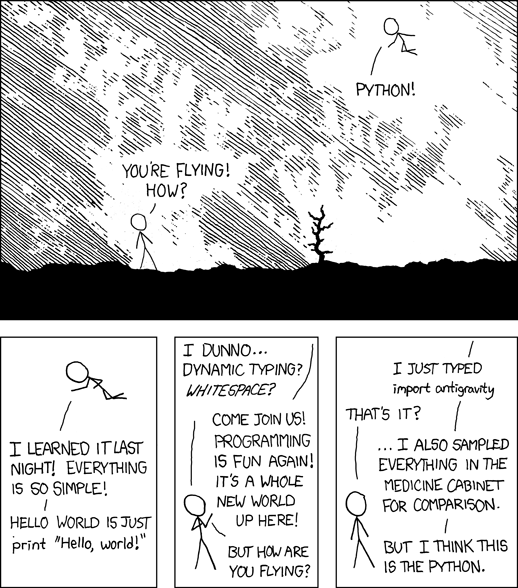
\includegraphics[width=0.6\linewidth]{figs/python_easy.png}}

\vspace{6mm}
\end{frame}

\section{Installation d'un environnement Python scientifique}

\begin{frame}[plain,fragile]
\frametitle{Installation d'un environnement Python scientifique}




\noindent\textbf{Qu’est ce que Anaconda ?}
L’installation d’un environnement Python complet peut-être une vraie galère. Déjà, il faut télécharger Python et l’installer. Par la suite, télécharger un à un les packages dont on a besoin. Parfois, le nombre de ces librairies peut-être grand.

Par ailleurs, il faut s’assurer de la compatibilité entre les versions des différentes packages qu’on a à télécharger. Bref, ce n’est pas amusant.


\end{frame}

\begin{frame}[plain,fragile]
% No title on this slide

\href{{https://www.anaconda.com/download/}}{Anaconda} est  une distribution Python. A son installation, Anaconda installera Python ainsi qu'une multitude de packages (voir \href{{https://docs.anaconda.com/anaconda/packages/pkg-docs#python-3-6}}{liste de packages anaconda}).  Cela nous évite de nous ruer dans les problèmes d’incompatibilités entre les différents packages.

Finalement, Anaconda propose un outil de gestion de packages appelé \href{{https://conda.io/docs/}}{conda}. Ce dernier permettra de mettre à jour et installer facilement les librairies dont on aura besoin pour nos développements.
\end{frame}

\begin{frame}[plain,fragile]
% No title on this slide

\noindent\textbf{Préparer la formation: téléchargement d’Anaconda.}
Nous demandons à tous les étudiants de télécharger Anaconda. Pour cela, il faut télécharger un installeur à partir de \href{{https://www.anaconda.com/download/}}{\nolinkurl{https://www.anaconda.com/download/}}, correspondant à votre système d’exploitation (Windows, Mac OS X, Linux). Il faut choisir entre 32 bits ou 64 bits (pour la version \emph{Python 3}) selon que votre système d’exploitation est 32 bits ou 64 bits.
\end{frame}

\begin{frame}[plain,fragile]
% No title on this slide

\begin{figure}[!ht]  % 
  \centerline{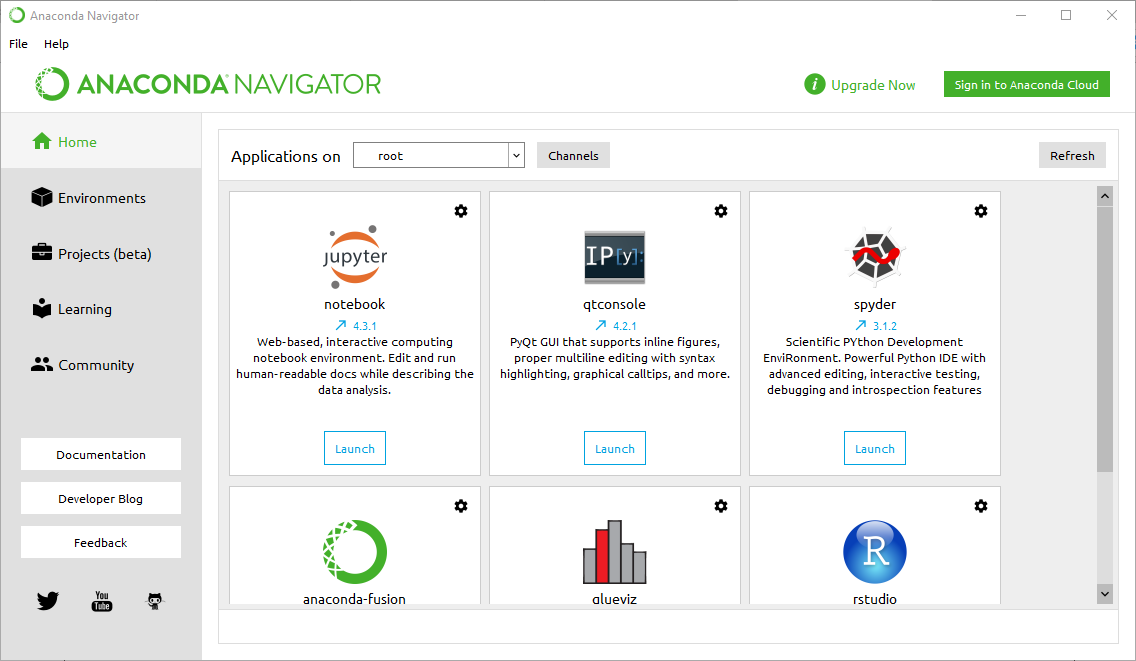
\includegraphics[width=0.7\linewidth]{figs/AnacondaNavigator.png}}
  \caption{
  Interface graphique du navigateur Anaconda sur Windows
  }
\end{figure}
%\clearpage % flush figures
\end{frame}

\begin{frame}[plain,fragile]
% No title on this slide

\begin{block}{Remarque}
Anaconda installe plusieurs exécutables pour développer en Python dans le répertoire \emph{anaconda/bin}, sans toujours créer des raccourcis sur le bureau ou dans un menu. Nous nous occuperons au tout début de la formation de créer des raccourcis pour pouvoir lancer l'application web \emph{Jupyter notebook}. Vous pouvez lancer le notebook depuis le navigateur Anaconda.
\end{block}
\end{frame}

\begin{frame}[plain,fragile]
\frametitle{Installation sur smartphone}

\noindent\textbf{Pydroid 3 - IDE éducatif pour Python 3.}
Pydroid 3 est l'IDE éducatif Python 3 le plus simple et le plus puissant à utiliser pour Android.

Pydroid 3 fournit:

\begin{itemize}
\item Interpréteur Python 3.6 hors connexion: Internet n'est pas nécessaire pour exécuter des programmes Python.

\item Pip package manager et un référentiel personnalisé pour les packages de roues prédéfinis pour les bibliothèques scientifiques améliorées, tels que numpy, scipy, matplotlib, scikit-learn et jupyter.

\item ...
\end{itemize}

\noindent
\end{frame}

\begin{frame}[plain,fragile]
% No title on this slide

\noindent\textbf{Installer et utiliser Pydroid 3 sur son smartphone:}

Pydroid est une application Android que vous pouvez obtenir sur Google Play: \href{{https://play.google.com/store/apps/details?id=ru.iiec.pydroid3}}{\nolinkurl{https://play.google.com/store/apps/details?id=ru.iiec.pydroid3}}

Les étapes suivantes, dans les figures ci-dessous, vous permettent d’utiliser le cahier Jupyter sur votre téléphone portable n’importe où et à tout moment pour vous entraîner au maximum et vous familiariser avec tous les exemples de programmation de ce cours.
\end{frame}

\begin{frame}[plain,fragile]
% No title on this slide

\textbf{Phase installation:}

1. Installer Pydroid 3 depuis Google Play: \href{{https://play.google.com/store/apps/details?id=ru.iiec.pydroid3}}{\nolinkurl{https://play.google.com/store/apps/details?id=ru.iiec.pydroid3}}

2. Ouvrez l'application, sur le menu cliquez sur pip et allez à l'onglet "QUICK INSTALL" pour obtenir les bibliothèques scientifiques nécessaires à ce cours.

3. Dans "QUICK INSTALL", installer les packages \emph{Jupyter} , \emph{numpy} et \emph{matplotlib}.


\begin{figure}[!ht]  % 
  \centerline{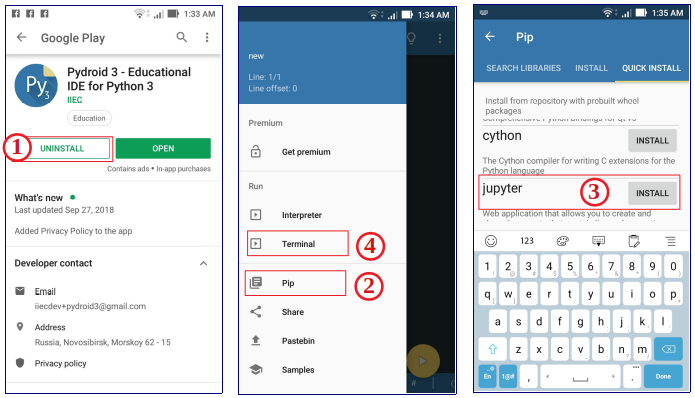
\includegraphics[width=0.7\linewidth]{figs/pydroid3_1.png}}
  \caption{
  Pydroid 3: Phase installation
  }
\end{figure}
%\clearpage % flush figures
\end{frame}

\begin{frame}[plain,fragile]
% No title on this slide

\textbf{Phase utilisation:}

4. Retournez au menu et ouvrez le \textbf{terminal}.

5. Sur le terminal, entrez la commande suivante:

\begin{minted}[fontsize=\fontsize{9pt}{9pt},linenos=false,mathescape,baselinestretch=1.0,fontfamily=tt,xleftmargin=2mm]{console}
jupyter notebook
\end{minted}

6. Jupyter s'exécutera sur votre navigateur Web. Accédez au répertoire dans lequel vous avez des notebooks à ouvrir, à télécharger (bouton \emph{upload}) ou à créer (bouton \emph{New}).

7. Amusez-vous à travailler sur le notebook: créez du contenu, lancez et modifiez des exemples


\begin{figure}[!ht]  % 
  \centerline{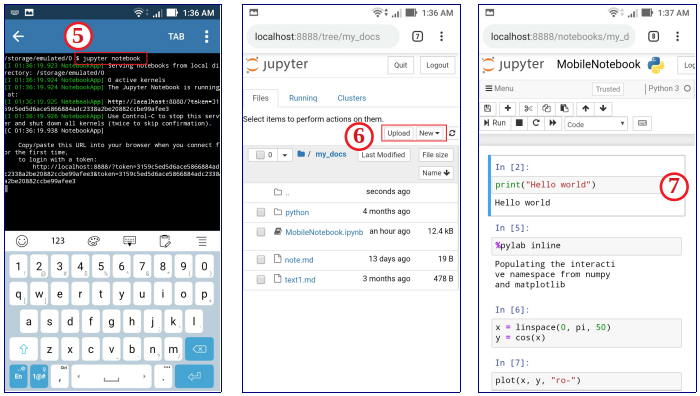
\includegraphics[width=0.7\linewidth]{figs/pydroid3_2.png}}
  \caption{
  Pydroid 3: Phase utilisation
  }
\end{figure}
%\clearpage % flush figures
\end{frame}

\section{PyEphem}

\begin{frame}[plain,fragile]
\frametitle{PyEphem}

Le module \textbf{PyEphem} (\href{{https://rhodesmill.org/pyephem/}}{\nolinkurl{https://rhodesmill.org/pyephem/}}) vous permet d'effectuer de nombreux calculs astronomiques professionnels. Vous pouvez l'utiliser:
\begin{itemize}
\item calculer les positions du soleil, de la lune, des planètes et de leurs lunes.

\item déterminer l'emplacement actuel des astéroïdes, des comètes et des satellites artificiels (fournir des éléments orbitaux).

\item déterminer le lever et le coucher du soleil d'objets divers en fonction de la position de l'observateur à la surface de la Terre.

\item trouver dans quelle constellation l'objet est.

\item calculer la position de étoiles, galaxies, etc.
\end{itemize}

\noindent
\textbf{PyEphem} est basé sur des procédures écrites pour le programme \textbf{XEphem} (\href{{www.clearskyinstitute.com/xephem/}}{\nolinkurl{www.clearskyinstitute.com/xephem/}}), disponible depuis de nombreuses années pour les utilisateurs du système \emph{Unix}.


\end{frame}

\begin{frame}[plain,fragile]
\frametitle{Installation}

La version 3.7.6.0 est la version la plus récente de PyEphem.


\vspace{6mm}

% inline figure
\centerline{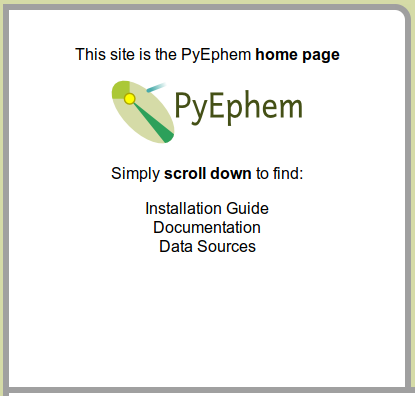
\includegraphics[width=0.3\linewidth]{figs/pyephem.png}}

\vspace{6mm}


Le moyen le plus simple d’installer PyEphem sur un ordinateur Window, Linux ou Mac OS, après s’être assuré que la distribution Python \textbf{Anaconda} est bien installée, est d'utiliser la commande \texttt{pip}, comme ceci:
\begin{minted}[fontsize=\fontsize{9pt}{9pt},linenos=false,mathescape,baselinestretch=1.0,fontfamily=tt,xleftmargin=2mm]{shell}
$ pip install pyephem
\end{minted}
\end{frame}

\begin{frame}[plain,fragile]
\frametitle{Importation de module et lieu de l'observateur}

Le module \textbf{PyEphem} est disponible sous le nom \textbf{ephem} qui peut être modifié lors de l’importation par l'alias \textbf{ep} pour raccourcir la programmation.
\begin{minted}[fontsize=\fontsize{9pt}{9pt},linenos=false,mathescape,baselinestretch=1.0,fontfamily=tt,xleftmargin=2mm]{python}
import ephem as ep
#OBSERVATEUR
obs = ep.Observer()
# nous créons une structure dans laquelle des données
# sur la position de l'observateur seront stockées
obs.lon = "10.00"
obs.lat = "36.5"
obs.name = "SAT-Tunis"
obs.elevation = 100.0
\end{minted}
Les fonctions et les structures du module \texttt{ephem } sont appelées dans la fonction \texttt{ep.method()}. Tout d'abord, nous définissons la position de l'observateur. Pour ce faire, nous créons la structure appropriée (\texttt{structure = ep.Observer()}) et remplissons ses champs (\texttt{structure.champ = valeur}).
\end{frame}

\begin{frame}[plain,fragile]
\frametitle{Objets célestes et leur localisation}

Tous les objets célestes importants tels que le Soleil, la Lune, les planètes et leurs lunes peuvent être créés par la structure de \texttt{fonction = ep.NomObjet()}.
\begin{minted}[fontsize=\fontsize{9pt}{9pt},linenos=false,mathescape,baselinestretch=1.0,fontfamily=tt,xleftmargin=2mm]{python}
# Objets
# nous créons une structure dans laquelle les données seront stockées
lune = ep.Moon()
\end{minted}
Après avoir créé l'objet, nous pouvons calculer son emplacement actuel en fournissant des informations sur l'observateur, situées dans la structure \texttt{obs} précédemment créée.
\begin{minted}[fontsize=\fontsize{9pt}{9pt},linenos=false,mathescape,baselinestretch=1.0,fontfamily=tt,xleftmargin=2mm]{python}
# CALCULS
# on calcule la position actuelle de l'objet
# pour l'observateur créé plus tôt
lune.compute(obs)
\end{minted}
Comme vous pouvez le constater, vous pouvez définir plusieurs observateurs différents et compter les coordonnées de l'objet sélectionné pour différents endroits de la Terre. Cela peut être utile lors de la planification de campagnes d’observation menées par différents observatoires.
\end{frame}

\begin{frame}[plain,fragile]
\frametitle{Lecture de coordonnées}

Les coordonnées calculées sont lues à partir des champs de structure d'objet.
\begin{minted}[fontsize=\fontsize{9pt}{9pt},linenos=false,mathescape,baselinestretch=1.0,fontfamily=tt,xleftmargin=2mm]{python}
# coordonnées calculées
print("Position actuelle de la Lune")
print(" ------------------------------ ")
# nous affichons l'ascension droite et la déclinaison
print("RA : ", lune.ra)
print("Dec : ", lune.dec)
# nous affichons l'azimut et l'élévation
print("--------------------------------")
print("Az : ", lune.az)
print ("El : " , lune.alt)
\end{minted}
Les valeurs calculées sont données au format \emph{\textbf{heures: minutes: secondes}} ou \emph{\textbf{degrés: minutes: secondes d'arc}} pour l'heure actuelle UT sur époque 2000.
\begin{Verbatim}[numbers=none,fontsize=\fontsize{9pt}{9pt},baselinestretch=0.95]
Position actuelle de la Lune
 ------------------------------
RA :  6:18:27.81
Dec :  20:49:04.9
--------------------------------
Az :  197:06:32.3
El :  56:50:39.8
\end{Verbatim}
\end{frame}

\begin{frame}[plain,fragile]
\frametitle{Coordonnées en degrés}

Toutes les coordonnées calculées par les procédures du module \textbf{PyEphem} sont données en \textbf{radians}. lorsque nous voulons écrire leur valeur, par exemple, les radians sont automatiquement convertis au format approprié (heures, minutes, secondes dans le cas d'une ascension droite ou degrés, minutes, secondes d'arc pour d'autres coordonnées).

Si vous souhaitez utiliser des coordonnées calculées sur un graphique, il est utile de les convertir en degrés à l'aide de la fonction degrés.

\begin{minted}[fontsize=\fontsize{9pt}{9pt},linenos=false,mathescape,baselinestretch=1.0,fontfamily=tt,xleftmargin=2mm]{python}
# coordonnées azimutales en degrés sous forme d'un nombre réel
print(" -------------------------------- ")
print("Az (deg): ", degrees(lune.az))
print("El (deg): ", degrees(lune.alt))
\end{minted}
Azimut et élévation en degrés:
\begin{Verbatim}[numbers=none,fontsize=\fontsize{9pt}{9pt},baselinestretch=0.95]
--------------------------------
Az (deg):  207.85208210454263
El (deg):  55.334644372169485
\end{Verbatim}
\end{frame}

\begin{frame}[plain,fragile]
\frametitle{Date et heure}

Nous pouvons attribuer n'importe quelle date et heure à chaque observateur:
\begin{minted}[fontsize=\fontsize{9pt}{9pt},linenos=false,mathescape,baselinestretch=1.0,fontfamily=tt,xleftmargin=2mm]{python}
# PROPRE DATE ET HEURE TU
obs.date = "2019/01/13 10:00:00"
\end{minted}
Il faut seulement se rappeler que les chiffres de la date sont séparés par le signe \texttt{/} et l'heure par deux points.
\end{frame}

\begin{frame}[plain,fragile]
\frametitle{Mouvement apparent du Soleil - le début du programme}

\begin{minted}[fontsize=\fontsize{9pt}{9pt},linenos=false,mathescape,baselinestretch=1.0,fontfamily=tt,xleftmargin=2mm]{python}
# IMPORTATION
from pylab import *
import ephem as ep
# OBSERVATEUR
obs = ep.Observer()
# TUNIS
obs.lon, obs.lat, obs.elev = '10.08', '36.4', 100.0
obs.name= "SAT-TUNIS"
# OBJET
soleil = ep.Sun()
# TEMPS
tm = linspace(0 , 24 , 25)
# GRAPHIQUE
pt = subplot(111 , polar= True )
\end{minted}
\end{frame}

\begin{frame}[plain,fragile]
\frametitle{Mouvement apparent du Soleil - solstice d'été}

\begin{minted}[fontsize=\fontsize{9pt}{9pt},linenos=false,mathescape,baselinestretch=1.0,fontfamily=tt,xleftmargin=2mm]{python}
# BOUCLE PRINCIPALE
for t in tm :
    # changement de temps
    obs.date = "2014/06/21 %02 d :00:00 "%t
    # on calcule les coordonnées
    sun.compute(obs)
    # coordonnées azimutales - azimut en radians
    az = float(repr(sun.az))
    el = degrees(float(repr(sun.alt)))
    # graphique - on change l'élévation par une distance zénithale
    pt.plot([az], [90 - el], ls =" ", marker= " o ", c =" yellow ", \
    markersize =10)
    # heure locale UTC +2 heures en été
    if el > 0:
        pt.text (az, 90 - el, " %02 d "%(t+2), fontsize =10, \
        ha = 'left' , va = 'center')
\end{minted}
\end{frame}

\begin{frame}[plain,fragile]
\frametitle{Mouvement apparent du Soleil - solstice d'hiver}

\begin{minted}[fontsize=\fontsize{9pt}{9pt},linenos=false,mathescape,baselinestretch=1.0,fontfamily=tt,xleftmargin=2mm]{python}
    # TRANSFERT HIVERNAL - nous répétons les calculs "en décembre"
    obs.date = "2014/12/22 %02d:00:00" % t
    soleil.compute(obs)
    az = float(repr(soleil.az))
    el = degrees(float(repr(soleil.alt)))
    pt.plot([az], [90 - el], ls ="", marker= "o", c ="blue", \
    markersize =10)
    # heure locale UTC +1 heures en hiver
    if el > 0:
        pt.text (az, 90 - el, "%02d"%(t+1), fontsize =10, \
        ha = 'left' , va = 'center')
# nous limitons la distance zénithale à 90 degrés - horizon
plt.set_rmax(90.0)
# nous plaçons le nord en haut du graphique
plt.set_theta_zero_location("N")
# ENGISTREZ LE GRAPHIQUE EN FORMAT PDF ET PNG
plt.savefig("figs/mvtSoleil.pdf"); plt.savefig ("figs/mvtSoleil.png")
plt.show ()
\end{minted}
\end{frame}

\begin{frame}[plain,fragile]
\frametitle{Mouvement apparent du Soleil - le graphique}

\vspace{6mm}

% inline figure
\centerline{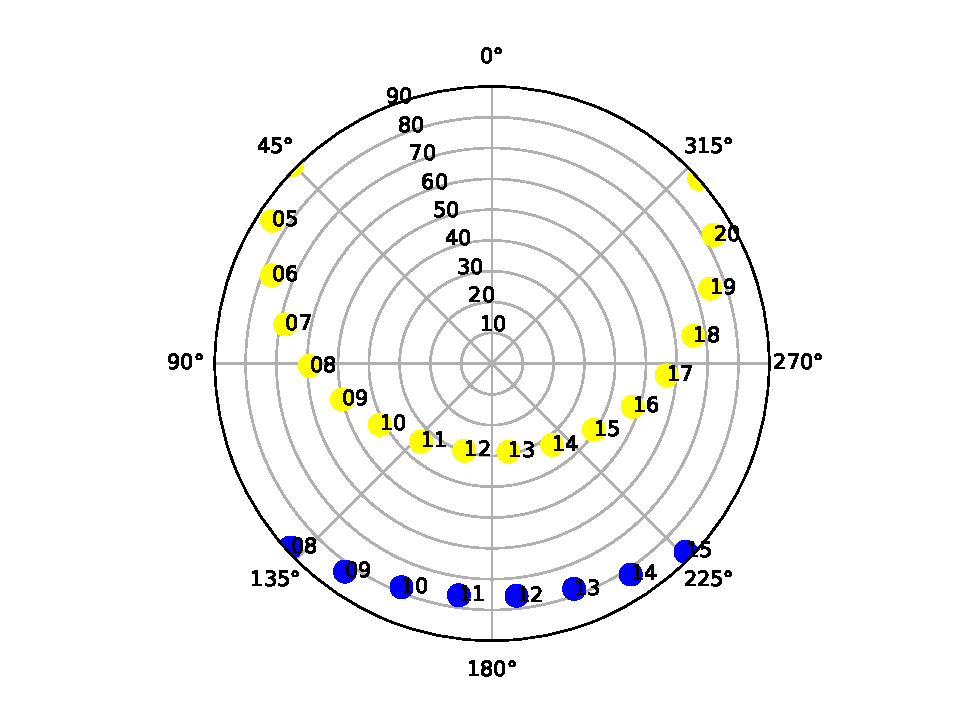
\includegraphics[width=0.9\linewidth]{figs/mvtSoleil.pdf}}

\vspace{6mm}
\end{frame}

\begin{frame}[plain,fragile]
% No title on this slide

% --- begin exercise ---
\begin{doconceexercise}
\refstepcounter{doconceexercisecounter}

\exercisesection{Exercise \thedoconceexercisecounter: Mouvement apparent du Soleil - région polaire}


Changer les coordonnées géographiques. Cette fois dans une ville proche de la région polaire et tracez le nouveau graphique. Que s'est-il passé et comment décrivez-vous le phénomène?

\end{doconceexercise}
% --- end exercise ---
\end{frame}

\begin{frame}[plain,fragile]
\frametitle{Mouvement rétrograde de Mars}

Dès l'Antiquité, il a été remarqué que le mouvement de certains objets dans le ciel est d'un caractère différent du trafic de la majorité (\textbf{étoiles fixes}). De tels objets ont été appelés étoiles errantes (\textbf{planètes}). Aujourd'hui, nous savons que errer sur les planètes a pour effet de placer leur mouvement en même temps que le mouvement de la Terre autour du Soleil. Nous pouvons retracer ce phénomène sur l'exemple de Mars.

\begin{figure}[!ht]  % 
  \centerline{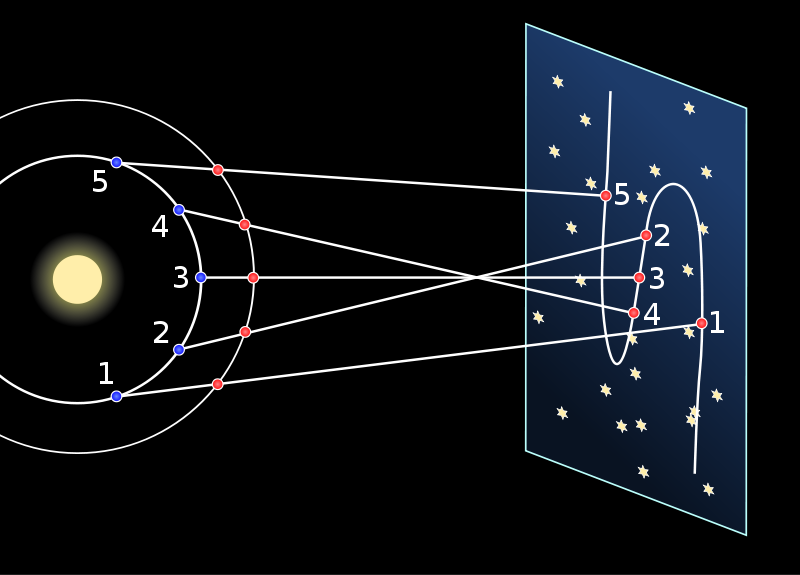
\includegraphics[width=0.5\linewidth]{figs/retro_mars.png}}
  \caption{
  Projetion depuis la Terre (en bleu) des mouvements de la planète extérieure (en rouge) sur la sphère des étoiles fixes. \emph{Source: Wikipédia}
  }
\end{figure}
%\clearpage % flush figures
\end{frame}

\begin{frame}[plain,fragile]
\frametitle{Mouvement rétrograde de Mars - début du programme}

\begin{minted}[fontsize=\fontsize{9pt}{9pt},linenos=false,mathescape,baselinestretch=1.0,fontfamily=tt,xleftmargin=2mm]{python}
# IMPORTATION
import ephem as ep
# deux fonctions supplémentaires du module datetime sont nécessaires
from datetime import datetime , timedelta

# OBSERVATEUR
obs = ep.Observer()
# COORDONNÉES DE TUNIS
obs.lon, obs.lat, obs.elev = '10.08', '36.4', 100.0
obs.name = "SAT-TUNIS"
# MARS
mr = ep.Mars()
\end{minted}
\end{frame}

\begin{frame}[plain,fragile]
\frametitle{Mouvement rétrograde de Mars - boucle principale}

\begin{minted}[fontsize=\fontsize{9pt}{9pt},linenos=false,mathescape,baselinestretch=1.0,fontfamily=tt,xleftmargin=2mm]{python}
from pylab import *
plt.figure(figsize=(10, 5))
for i in range (0 , 181):
    # nous changeons la date d'un jour pendant six mois
    dt = datetime (2018, 5, 1) + timedelta(i)
    ds = "%d/%02d/%02d"%(dt.year, dt.month, dt.day)
    print(" jour de l'année: ", i +1 , ds)
    # fixer la date de l'observateur et calculer les coordonnées
    obs.date = ds
    mr.compute(obs)
    ra = degrees(float(repr(mr.ra)))
    de = degrees(float(repr(mr.dec)))
    # on dessine des objets
    plot([ra], [de], c = "red", marker = "o", alpha =.5)
    # nous ajoutons une description de la date en moyenne tous les 10 jours
    if (dt.day % 10) == 0: text(ra, de, ds, fontsize =8)

# description du graphique
xlabel("ascension droite " + r"$\alpha$ (deg)")
ylabel(" déclinaison " + r"$\delta$ (deg)")
title("Mouvement retrograde de Mars - 6 mois en 2018 \n"+obs.name, fontweight='bold')
savefig("../figs/retrogradeMars.pdf"); savefig("../figs/retrogradeMars.png")
show()
\end{minted}
\end{frame}

\begin{frame}[plain,fragile]
\frametitle{Mouvement rétrograde de Mars - le graphique}

\vspace{6mm}

% inline figure
\centerline{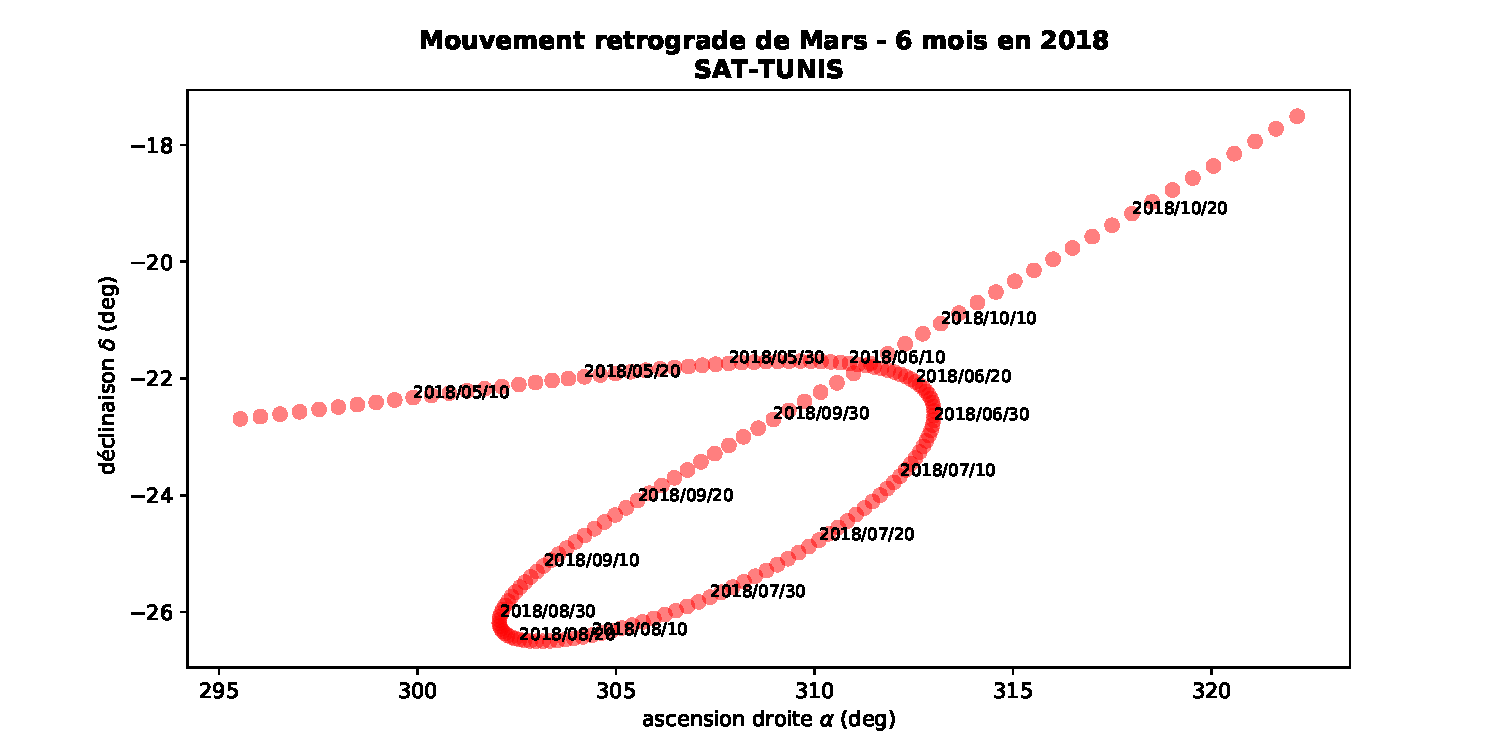
\includegraphics[width=0.9\linewidth]{figs/retrogradeMars1.pdf}}

\vspace{6mm}
\end{frame}

\begin{frame}[plain,fragile]
\frametitle{Mouvement rétrograde de Mars - changement du texte des axes}

\begin{minted}[fontsize=\fontsize{9pt}{9pt},linenos=false,mathescape,baselinestretch=1.0,fontfamily=tt,xleftmargin=2mm]{python}
# conversion RA donné en degrés
# sur les formats heure, minute et seconde
def RAd2hms (x, loc):
    h = x//15
    m = int(((x - h * 15.0) / 15.0) * 60.0)
    s = ((x - h *15 - m / 4.0) / 15.0) * 3600.0
    return "%02dh%02dm%02ds"%(h, m, s)
# changement de déclinaison donné en degrés
# le format du degré, minute, second arc
def DEd2dms (x , loc ):
    d = int(fabs(x))
    m = int((fabs(x) - d)*60)
    s = (fabs(x) - d - m /60.0)*3600.0
    if x <0: d = -1 * d
    return " %02dd%02dm%02ds"%(d, m, s)

# description du graphique
xlabel("ascension droite " + r"$\alpha$")
gca().xaxis.set_major_formatter(FuncFormatter(RAd2hms))
ylabel(" déclinaison " + r"$\delta$")
gca().yaxis.set_major_formatter(FuncFormatter(DEd2dms))
title("Mouvement retrograde de Mars - 6 mois en 2018 \n"+obs.name, fontweight='bold')

savefig("../figs/retrogradeMars.pdf"); savefig("../figs/retrogradeMars.png")
show()
\end{minted}
\end{frame}

\begin{frame}[plain,fragile]
\frametitle{Mouvement rétrograde de Mars - le graphique}

\vspace{6mm}

% inline figure
\centerline{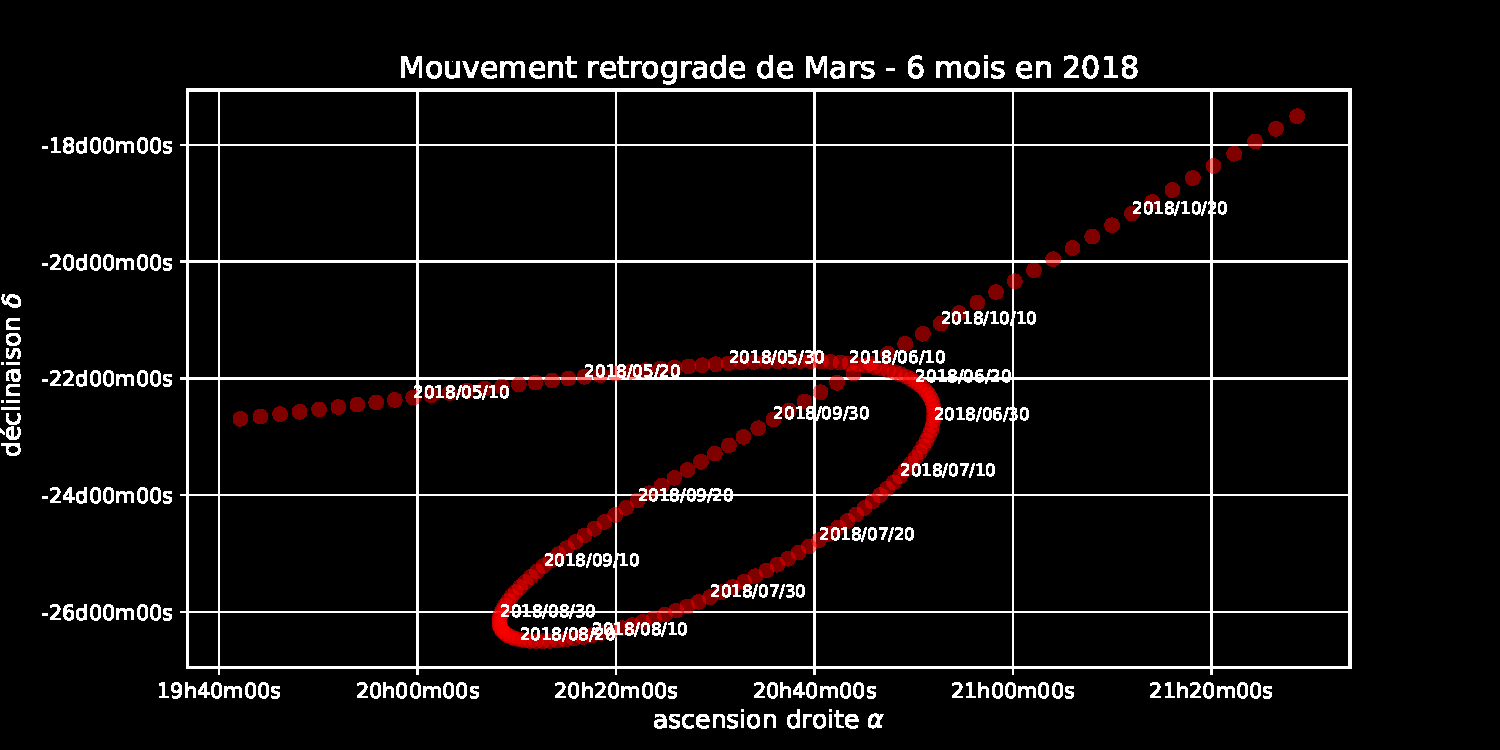
\includegraphics[width=0.9\linewidth]{figs/retrogradeMars.pdf}}

\vspace{6mm}
\end{frame}

\begin{frame}[plain,fragile]
% No title on this slide

% --- begin exercise ---
\begin{doconceexercise}
\refstepcounter{doconceexercisecounter}

\exercisesection{Exercise \thedoconceexercisecounter: Quand le prochain mouvement rétrograde de la planète Mars?}


Changez la période et trouvez le prochain mouvement rétrograde de la planète Mars.

\end{doconceexercise}
% --- end exercise ---
\end{frame}

\begin{frame}[plain,fragile]
\frametitle{Mouvement des lunes galiléennes - début du programme}

\begin{minted}[fontsize=\fontsize{9pt}{9pt},linenos=false,mathescape,baselinestretch=1.0,fontfamily=tt,xleftmargin=2mm]{python}
# IMPORTATION
import ephem as ep
# NOUS CRÉONS LES OBJETS
Io = ep.Io()
Eu = ep.Europa()
Ga = ep.Ganymede()
Ca = ep.Callisto()
# Créons des tableaux vide pour
# SAUVEGARDER LES COORDONNÉES
y = []
xIo = []
xEu = []
xGa = []
xCa = []
\end{minted}
\end{frame}

\begin{frame}[plain,fragile]
\frametitle{Mouvement des lunes galiléennes - boucle principale}

\begin{minted}[fontsize=\fontsize{9pt}{9pt},linenos=false,mathescape,baselinestretch=1.0,fontfamily=tt,xleftmargin=2mm]{python}
# pas de temps - heure
dt = ep.hour
# temps initial
ts = ep.now()
# heure actuelle
tm = ts
N=2*24
for i in range(N):
    # nous calculons des valeurs y
    y.append((tm - ts)*24.0)
    # nous calculons des valeurs x
    Io.compute(tm)
    Eu.compute(tm)
    Ga.compute(tm)
    Ca.compute(tm)
    # nous ajoutons des calculs aux tableaux
    xIo.append(Io.x)
    xEu.append(Eu.x)
    xGa.append(Ga.x)
    xCa.append(Ca.x)
    # on augmente le temps d'une heure
    tm += dt
\end{minted}
\end{frame}

\begin{frame}[plain,fragile]
\frametitle{Mouvement des lunes galiléennes - le graphique}

\begin{minted}[fontsize=\fontsize{9pt}{9pt},linenos=false,mathescape,baselinestretch=1.0,fontfamily=tt,xleftmargin=2mm]{python}
from pylab import *
fig1 = plt.figure()
plot(xIo, y, marker ="o", label ="Io")
plot(xEu, y, marker ="o", label ="Europa")
plot(xGa, y, marker ="o", label ="Ganimedes")
plot(xCa, y, marker ="o", label ="Callisto")
plot(zeros(len(y)),y ,marker =r"$\mathcircled{J}$", markersize =15,
     label ="Jupiter",color ="orange", fillstyle= 'none')
xlabel(u"position par rapport à Jupiter")
ylabel("Heures à partir de (%s TU)"% ts)
ylim(0,N+3)
title(u"Mouvement des lunes galiléennes")
grid()
legend(loc =1)

tight_layout()
savefig("../figs/mvtjov.pdf"); savefig("../figs/mvtjov.png")
show()
\end{minted}
\end{frame}

\begin{frame}[plain,fragile]
\frametitle{Mouvement des lunes galiléennes - le graphique}

\vspace{6mm}

% inline figure
\centerline{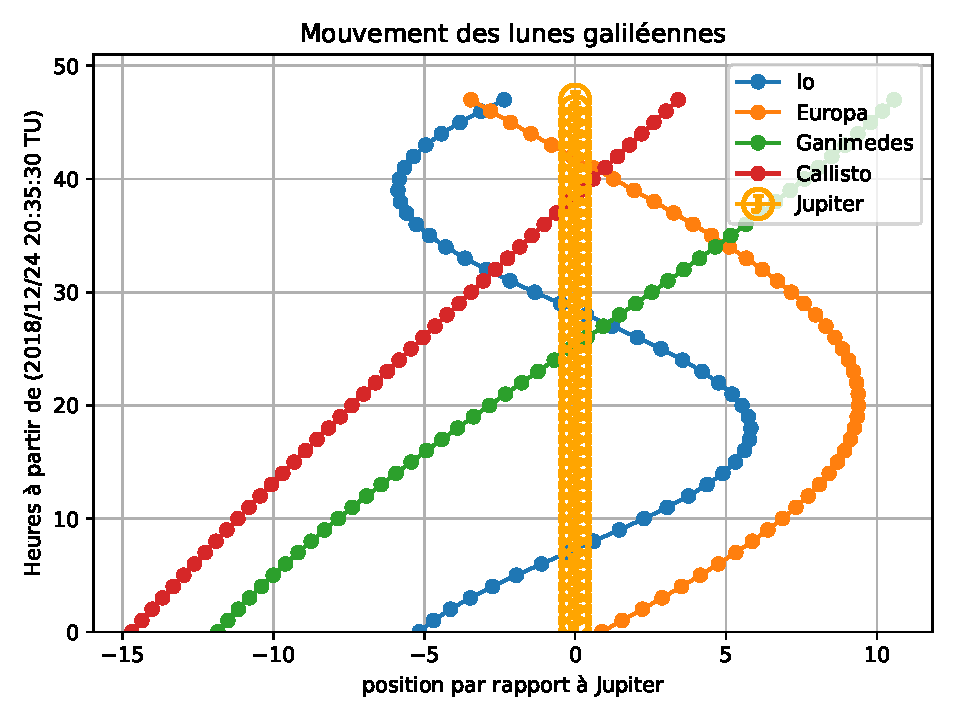
\includegraphics[width=0.9\linewidth]{figs/mvtjov.pdf}}

\vspace{6mm}
\end{frame}

\begin{frame}[plain,fragile]
\frametitle{Détermination de l'éclipse solaire - début du programme}

\begin{minted}[fontsize=\fontsize{9pt}{9pt},linenos=false,mathescape,baselinestretch=1.0,fontfamily=tt,xleftmargin=2mm]{python}
# IMPORTATION
import ephem as ep
# OBSERVATEUR
obs = ep.Observer()
obs.lon, obs.lat, obs.elev = '10.08', '36.4', 100.0
obs.name = "SAT-TUNIS"
# OBJETSNIS
soleil = ep.Sun()
lune = ep.Moon()
# pas de temps - heure
dt = ep.hour
# temps initial
#ts = ep.now()
ts=ep.Date("2015-01-01 00:00:00")
# heure actuelle
tm = ts
\end{minted}
\end{frame}

\begin{frame}[plain,fragile]
\frametitle{Détermination de l'éclipse solaire - boucle principale}

Nous vérifions la séparation du soleil et de la lune toutes les heures pendant les 10 prochaines années.
\begin{minted}[fontsize=\fontsize{9pt}{9pt},linenos=false,mathescape,baselinestretch=1.0,fontfamily=tt,xleftmargin=2mm]{python}
for i in range (365*24*10):
    # nous fixons l'heure actuelle
    obs.date = tm
    # nous calculons les coordonnées
    soleil.compute(obs)
    lune.compute(obs)
    # rayons
    rs = soleil.radius
    rl = lune.radius
    # on calcule la distance angulaire
    sp = ep.separation(soleil, lune)
    # on vérifie si la somme des rayons sera inférieure
    # à la séparation calculée
    if sp < rs + rl :
    # nous vérifions si le soleil sera au-dessus de l'horizon
        if soleil.alt > 0.0:
            print("Date de l'eclipse UT: ", ep.Date(tm), "Separation: ", sp)
    # on augmente le temps par pas d'une heure
    tm += dt
\end{minted}
\end{frame}

\begin{frame}[plain,fragile]
\frametitle{Détermination de l'éclipse solaire -}

Les dates de l'éclipse solaire planifiée visible de la Tunisie au cours des 10 prochaines années.
\begin{Verbatim}[numbers=none,fontsize=\fontsize{9pt}{9pt},baselinestretch=0.95]
Date de l'eclipse UT:  2020/6/21 05:00:00 Separation:  0:30:50.0
Date de l'eclipse UT:  2022/10/25 10:00:00 Separation:  0:29:25.7
Date de l'eclipse UT:  2022/10/25 11:00:00 Separation:  0:30:51.9
Date de l'eclipse UT:  2025/3/29 11:00:00 Separation:  0:32:49.2
Date de l'eclipse UT:  2026/8/12 18:00:00 Separation:  0:20:53.8
Date de l'eclipse UT:  2027/8/2 08:00:00 Separation:  0:30:44.7
Date de l'eclipse UT:  2027/8/2 09:00:00 Separation:  0:04:33.3
Date de l'eclipse UT:  2027/8/2 10:00:00 Separation:  0:21:01.3
Date de l'eclipse UT:  2028/1/26 16:00:00 Separation:  0:26:09.8
\end{Verbatim}
\end{frame}

\begin{frame}[plain,fragile]
\frametitle{Phases d'une éclipse solaire - début du programme}

\begin{minted}[fontsize=\fontsize{9pt}{9pt},linenos=false,mathescape,baselinestretch=1.0,fontfamily=tt,xleftmargin=2mm]{python}
# IMPORTATION
from pylab import *
import ephem as ep
# OBSERVATEUR
obs = ep.Observer()
# TUNIS
obs.lon, obs.lat, obs.elev = '10.08', '36.4', 100.0
obs.name= "SAT-TUNIS"
# CRÉER DES OBJETS
soleil = ep.Sun()
lune = ep.Moon()
# intervalle de temps - 20 minutes
dt = ep.hour/4.
# TEMPS DE DÉBUT
ts = ep.Date("2027-08-02 08:00:00")
obs.date = ts
# nous calculons les coordonnées
soleil.compute(obs)
lune.compute(obs)
rs = degrees(soleil.radius)
rl = degrees(lune.radius )
\end{minted}
\end{frame}

\begin{frame}[plain,fragile]
\frametitle{Phases d'une éclipse solaire - suite}

\begin{minted}[fontsize=\fontsize{9pt}{9pt},linenos=false,mathescape,baselinestretch=1.0,fontfamily=tt,xleftmargin=2mm]{python}
# nous calculons les coordonnées
soleil.compute(obs)
lune.compute(obs)
rs = degrees(soleil.radius)
rl = degrees(lune.radius )

# Nous créons un graphique en l'attribuant à un pl COMME variable
fig=plt.figure(figsize=(6,5))
pl = subplot(111, aspect ="equal")
# titre du graphique avec date et heure
pl.set_title (obs.name+"\n début en (TU): "+str(ep.Date(ts)))
# Nous nous plaçons le soleil dans le centre
sc=Circle((0 ,0), rs, facecolor ="yellow",
            edgecolor ="red", lw =2)

pl.add_artist(sc)
# les coordonnées du Soleil
pl.text(0, rs+0.1, "Az: %.1f, El: %.1f"%(degrees(soleil.az), degrees(soleil.alt)),
        ha='center', fontsize =14)
\end{minted}
\end{frame}

\begin{frame}[plain,fragile]
\frametitle{Phases d'une éclipse solaire - boucle principale}

\begin{minted}[fontsize=\fontsize{9pt}{9pt},linenos=false,mathescape,baselinestretch=1.0,fontfamily=tt,xleftmargin=2mm]{python}
# Nous plaçons la Lune dans la figure
for i in range(10):
    print("time UT: ", ep.Date(ts))
    obs.date = ts
    # nous calculons les coordonnées
    soleil.compute(obs)
    lune.compute(obs)
    # Nous calculons la différence de position
    az = degrees(soleil.az - lune.az)
    el = degrees(soleil.alt - lune.alt)
    # dessiner et la position réelle en empillements d'image de Lune; le Soleil estau centre
    kc = Circle((az , el), rl , facecolor ="gray",
                edgecolor ="black", lw =2, alpha =0.3)
    pl.add_artist(kc)
    # augmenter le temps de 20 minutes
    ts += dt

pl.set_xlim (-1.0, 1.0)
pl.set_ylim (-1.0, 1.0)
pl.set_xlabel ("degré")
pl. set_ylabel ("degré")
plt.tight_layout()
savefig("../figs/eclipse_sol_" + str(ts) +".pdf"); savefig("../figs/eclipse_sol_" + str(ts) +".png")
show ()
\end{minted}
\end{frame}

\begin{frame}[plain,fragile]
\frametitle{Phases d'une éclipse solaire - le graphique}

\vspace{6mm}

% inline figure
\centerline{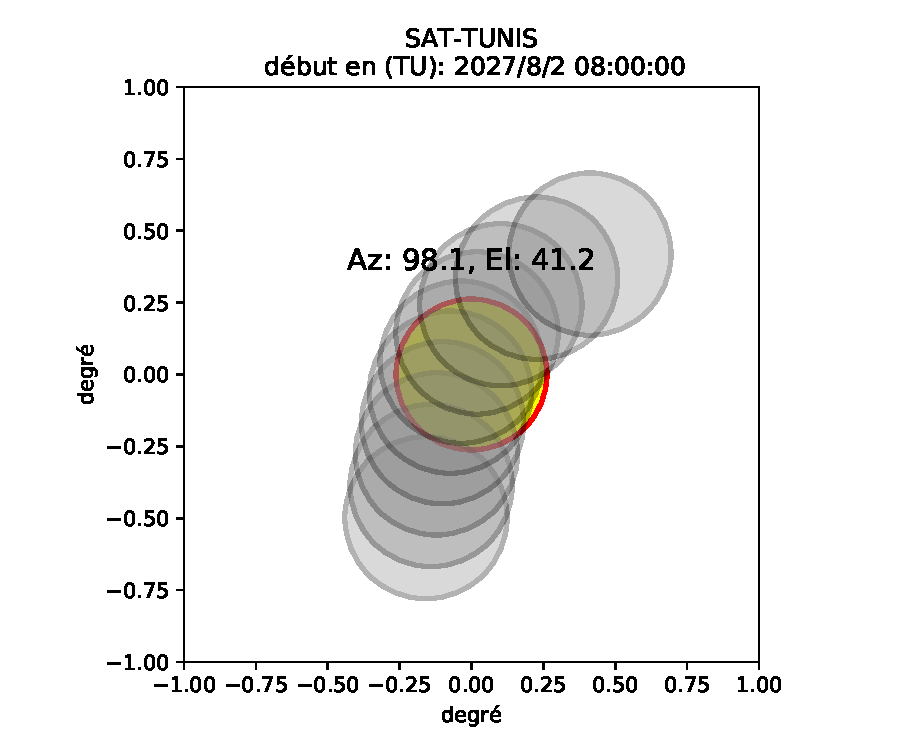
\includegraphics[width=0.9\linewidth]{figs/eclipse_sol.pdf}}

\vspace{6mm}
\end{frame}

\begin{frame}[plain,fragile]
\frametitle{Conjonction de la lune et des planètes}

\begin{minted}[fontsize=\fontsize{9pt}{9pt},linenos=false,mathescape,baselinestretch=1.0,fontfamily=tt,xleftmargin=2mm]{python}
# IMPORTOWANIE
from pylab import *
import ephem as ep
# OBSERVATEUR
obs = ep.Observer()
# TUNIS
obs.lon, obs.lat, obs.elev = '10.08', '36.4', 100.0
obs.name= "SAT-TUNIS"
# NOUS CRÉONS UN OBJET
# on vérifie si c'est sous l'horizon
soleil = ep.Sun()
lune = ep.Moon()
venus = ep.Venus()
mars = ep.Mars()
jupiter = ep.Jupiter()
# pas de temps - heure
dt = ep.hour
# temps initial
ts = ep.now()
# heure actuelle
tm = ts
\end{minted}
\end{frame}

\begin{frame}[plain,fragile]
\frametitle{Conjonction de la lune et des planètes - boucle principale}

\begin{minted}[fontsize=\fontsize{9pt}{9pt},linenos=false,mathescape,baselinestretch=1.0,fontfamily=tt,xleftmargin=2mm]{python}
# BOUCLE PRINCIPAL DU PROGRAMME
for i in range (365*24*1):
# nous fixons l'heure actuelle
    obs.date = tm
    # nous calculons des coordonnées
    soleil.compute(obs)
    lune.compute(obs)
    venus.compute(obs)
    mars.compute(obs)
    jupiter.compute(obs)
    # on calcule la séparation
    s1 = ep.separation(venus , lune)
    s2 = ep.separation(mars , lune)
    s3 = ep.separation(jupiter , lune)
    # la séparation doit être inférieure à 5 degrés
    if degrees(s1) < 5:
        # nous vérifions si la lune sera au-dessus de l'horizon
        # et si le soleil est au-dessous de l'horizon
        if degrees(lune.alt) > 5.0 and degrees(soleil.alt) < -5.0:
            print("-------------------------------------------------------------")
            print(u"précédente nouvelle lune , UT :", ep.previous_new_moon(ep.Date(tm)))
            print(u"Vénus - Lune , UT :", ep.Date(tm) ,"séparation :", s1)
            print(u"pos. Lune :", lune.az ,"El :", lune.alt)
\end{minted}
\end{frame}

\begin{frame}[plain,fragile]
\frametitle{Conjonction de la lune et des planètes - boucle principale (suite)}

\begin{minted}[fontsize=\fontsize{9pt}{9pt},linenos=false,mathescape,baselinestretch=1.0,fontfamily=tt,xleftmargin=2mm]{python}
if degrees(s2) < 5:
    if degrees(lune.alt) > 5.0 and degrees(soleil.alt) < -5.0:
        print("------------------------------------------------------------------")
        print(u"précédente nouvelle lune , UT :", ep.previous_new_moon(ep.Date(tm)))
        print(u"Mars - Lune , UT :", ep.Date(tm) ,"séparation :", s2)
        print(u"Pos. Lune, Az :", lune.az ,"El :", lune.alt)
if degrees(s3) < 5:
    if degrees(lune.alt) > 5.0 and degrees(soleil.alt) < -5.0:
        print("--------------------------------------------------------------")
        print(u"précédente nouvelle lune , UT :", ep.previous_new_moon(ep.Date(tm)))
        print(u"Jupiter - Lune , UT :", ep.Date(tm) ,"séparation :", s3)
        print(u"Pos. Lune, Az :", lune.az ,"El :", lune.alt)
    # on augmente le temps d'une heure
tm += dt
\end{minted}

Exemples de résultats de calculs:

\begin{Verbatim}[numbers=none,fontsize=\fontsize{9pt}{9pt},baselinestretch=0.95]
--------------------------------------------------------------
précédente nouvelle lune , UT : 2019/1/6 01:28:11
Jupiter - Lune , UT : 2019/1/31 03:47:21 séparation : 3:09:07.3
Pos. Lune, Az : 122:58:36.9 El : 8:18:03.0
--------------------------------------------------------------
précédente nouvelle lune , UT : 2019/2/4 21:03:35
Vénus - Lune , UT : 2019/3/3 04:47:21 séparation : 4:07:18.5
pos. Lune : 121:01:33.3 El : 6:15:18.7
--------------------------------------------------------------
\end{Verbatim}
\end{frame}

\section{Cartopy}

\begin{frame}[plain,fragile]
\frametitle{Cartopy}

\textbf{Cartopy} est un package Python conçu pour le traitement des données géospatiales afin de produire des cartes et d’autres analyses de données géospatiales.

\textbf{Installation de Cartopy:}

Le moyen le plus simple d’installer \textbf{Cartopy} est \textbf{Conda}. Pour toutes les plateformes, l’installation de cartopy peut se faire avec:
\begin{minted}[fontsize=\fontsize{9pt}{9pt},linenos=false,mathescape,baselinestretch=1.0,fontfamily=tt,xleftmargin=2mm]{shell}
conda install -c conda-forge cartopy
\end{minted}

\textbf{Exemple simple:}

\begin{minted}[fontsize=\fontsize{9pt}{9pt},linenos=false,mathescape,baselinestretch=1.0,fontfamily=tt,xleftmargin=2mm]{python}
import datetime
import matplotlib.pyplot as plt
import cartopy.crs as ccrs
from cartopy.feature.nightshade import Nightshade
fig = plt.figure(figsize=(10, 5))
ax = fig.add_subplot(1, 1, 1, projection=ccrs.PlateCarree())
date = datetime.datetime(2019, 1, 13, 11)
ax.set_title('Night time shading for {}'.format(date))
ax.stock_img()
ax.add_feature(Nightshade(date, alpha=0.2))
plt.show()
\end{minted}


\end{frame}

\begin{frame}[plain,fragile]
\frametitle{Graphique}

\vspace{6mm}

% inline figure
\centerline{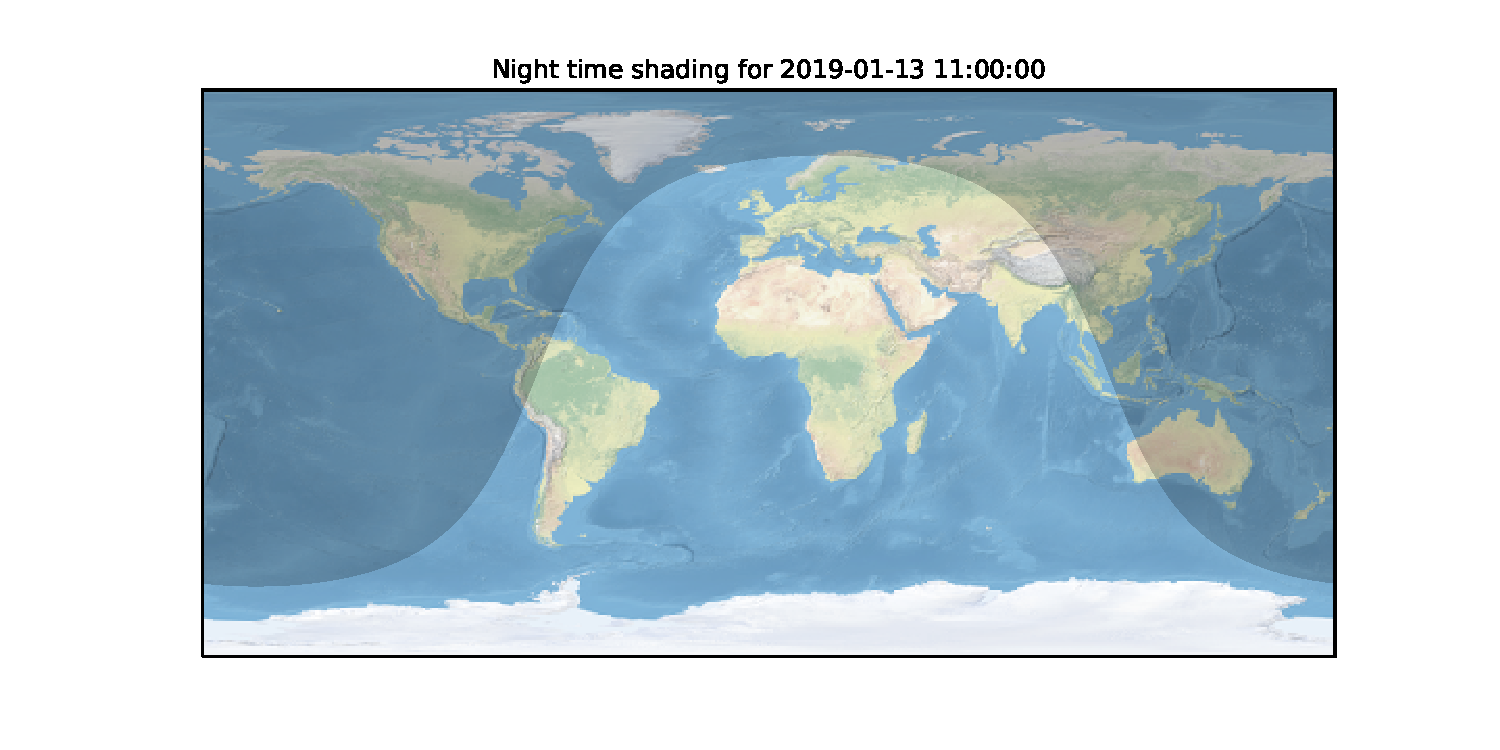
\includegraphics[width=1.2\linewidth]{figs/cartopy1.pdf}}

\vspace{6mm}
\end{frame}

\begin{frame}[plain,fragile]
\frametitle{Application: Eclipse totale du Soleil en 2027}

\vspace{6mm}

% inline figure
\centerline{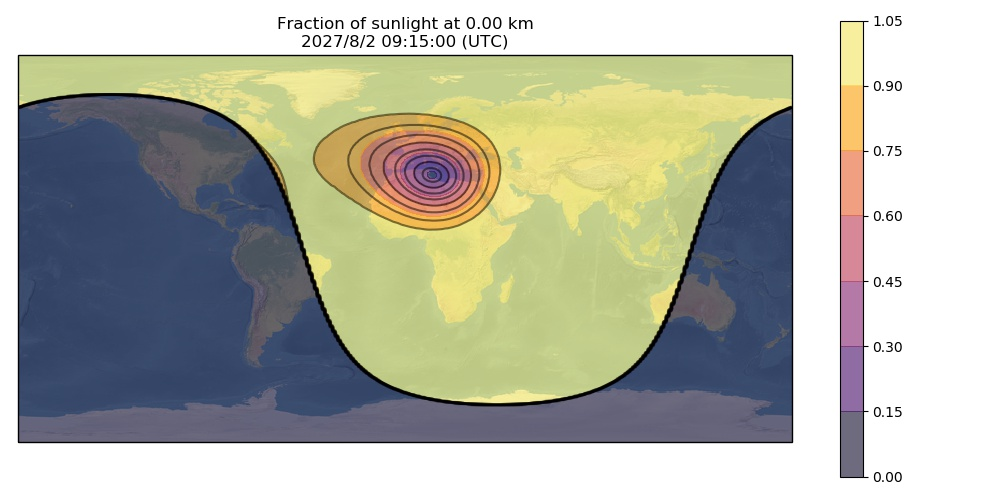
\includegraphics[width=1.1\linewidth]{figs/eclipse-4659.jpg}}

\vspace{6mm}
\end{frame}

\begin{frame}[plain,fragile]
% No title on this slide

\textbf{Merci de votre attention!}
\end{frame}

\end{document}
